\chapter{Présentation et installation}
%%%%%%%%%%%%%%%%%%%%%%%%%%%%%%%%%%
%
%%%%%%%%%%%%%%%%%%%%%%%%%%%%%%%%%%

\section{Présentation des simulateurs}
%
Les simulateurs SiCP, SiCF et SiGP sont des programmes informatiques écrit en C et utilisant la librairie SDL. Ils donnent une représentation graphique des phénomènes physiques simulés numériquement. Ils permettent également de faire varier les paramètres physiques de manière dynamique.
%
\subsection{SiCF et SiCP, simulateurs d'oscillateurs couplés}
%
SiCF et SiCP sont des simulateurs d'oscillateurs couplés à une dimension. Ils possèdent un certain nombre de caractéristiques communes : 

\begin{itemize}[leftmargin=1cm, label=\ding{32}, itemsep=0pt]
\item Représentation graphique des systèmes physiques simulés,
\item Modification dynamique des paramètres physiques,
\item Moteur sinusoïdale, carré, ou impulsionnelle,
\item Conditions aux limites peuvent être périodique, libre ou fixe.
\end{itemize}
%
\subsection{SiCF, corde vibrante et transformée de fourier}
%
\begin{center}
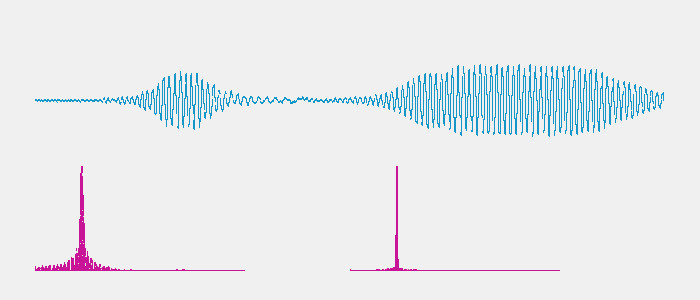
\includegraphics[scale=0.51]{./titre/heisenberg2}
\end{center}
%
\begin{itemize}[leftmargin=1cm, label=\ding{32}, itemsep=0pt]
\item Simulation numérique d'une corde vibrante.
\item Représentation graphique de la corde.
\item Calcul de la transformée de fourier.
\item Représentation du spectre.
\item Enregistrement et rechargement des situations.
\item Conditions initiales préenregistrées.
\end{itemize}
%
\subsection{SiCP, chaîne de pendules couplés}
%
\begin{center}
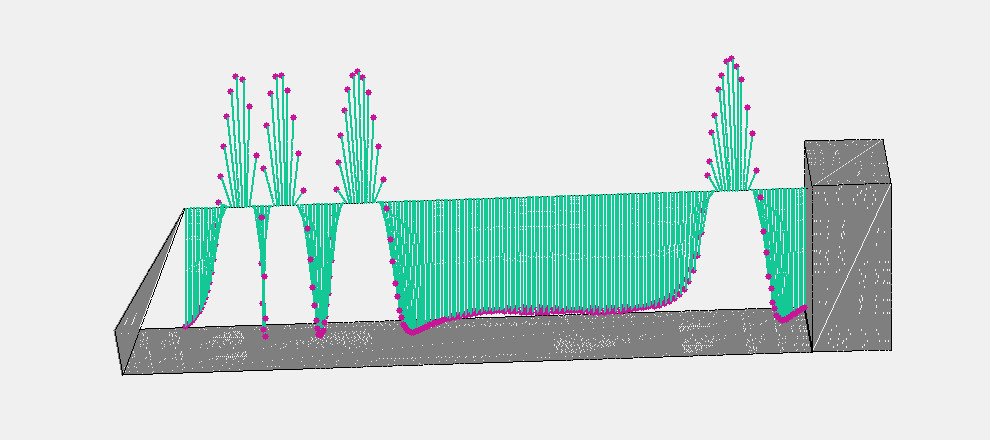
\includegraphics[scale=0.41]{./titre/SiCP}
\end{center}
%
\begin{itemize}[leftmargin=1cm, label=\ding{32}, itemsep=0pt]
\item Nombre de pendule variable.
\item Simulation de l'équation de sine-gordon et du courant josephson.
\item Graphisme en 3 dimensions, déplacement du point du vue.
\end{itemize}
%
\subsection{SiGP, thermodynamique statistique}
%
Le simulateur de gaz parfait SiGP permet de visualiser une interprétation statistique de la détente de Joule, du démon de Maxwell ainsi que du contact avec un ou deux thermostats.
%
\begin{center}
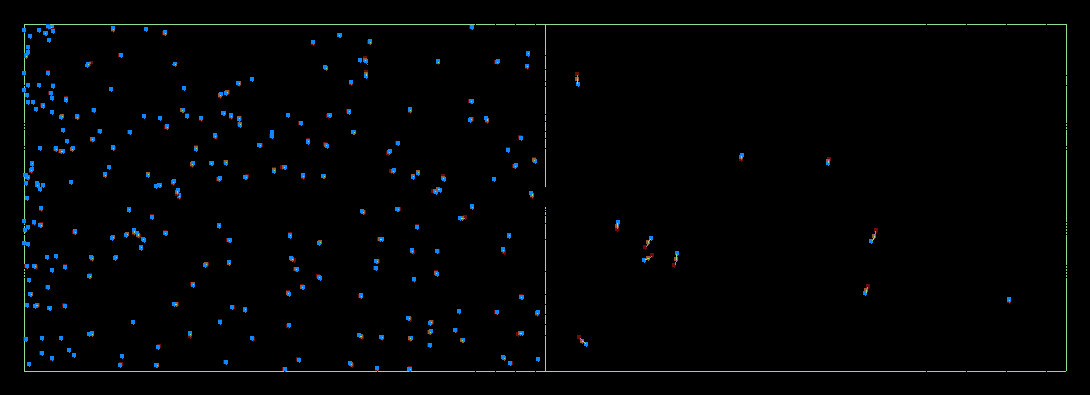
\includegraphics[scale=0.41]{./titre/SiGP}
\end{center}
%
\begin{itemize}[leftmargin=1cm, label=\ding{32}, itemsep=0pt]
\item Simulation de collisions élastiques.
\item Représentation graphique. 
\item Ajustement de la température des parois.
\item Paroi centrale et détente de joule.
\item Paroi centrale et démon de Maxwel.
\end{itemize}
%
%
\section{Installation des simulateurs}
Cette section traite de l'installation des simulateurs SiGP, SiCF et SiCP sur un système d'exploitation de type debian. Le téléchargement se fait avec un navigateur internet, la compilation et l'exécution se font dans un terminal. L'installation des outils de compilation nécessite les privilèges du super-utilisateur.
\begin{itemize}[leftmargin=1cm, label=\ding{32}, itemsep=0pt]
\item {\bf Installation des outils de compilation}
	\begin{itemize}[leftmargin=1cm, label=\ding{32}, itemsep=0pt]
	\item \texttt{sudo apt-get install gcc make libsdl-dev}
	\end{itemize}
\item {\bf Téléchargement des sources}
	\begin{itemize}[leftmargin=1cm, label=\ding{32}, itemsep=0pt]
	\item Télécharger les fichiers \texttt{.zip} sur github
		\begin{itemize}[leftmargin=1cm, label=\ding{32}, itemsep=0pt]
		\item \texttt{https://github.com/runigo/SiCP/archive/master.zip}
		\item \texttt{https://github.com/runigo/SiCF/archive/master.zip}
		\item \texttt{https://github.com/runigo/SiGP/archive/master.zip}
		\end{itemize}
	\item Décompresser les fichiers \texttt{.zip}
		\begin{itemize}[leftmargin=1cm, label=\ding{32}, itemsep=0pt]
		\item \texttt{unzip SiCP-master.zip}
		\item \texttt{unzip SiCF-master.zip}
		\item \texttt{unzip SiGP-master.zip}
		\end{itemize}
	\end{itemize}
\item {\bf Compilation}
	\begin{itemize}[leftmargin=1cm, label=\ding{32}, itemsep=0pt]
	\item La commande \texttt{make} dans le répertoire des sources produit un fichier exécutable :
		\begin{itemize}[leftmargin=1cm, label=\ding{32}, itemsep=0pt]
		\item \texttt{SiCF} pour SiCF
		\item \texttt{SiCP} pour SiCP
		\item \texttt{SiGP} pour SiGP
		\end{itemize}
	\end{itemize}

\item {\bf Exécution}
	\begin{itemize}[leftmargin=1cm, label=\ding{32}, itemsep=0pt]
	\item En ligne de commande, avec d'éventuelles options
		\begin{itemize}[leftmargin=1cm, label=\ding{32}, itemsep=0pt]
		\item \texttt{./SiCF [OPTION]}
		\item \texttt{./SiCP [OPTION]}
		\item \texttt{./SiGP [OPTION]}
		\end{itemize}
	\item La fenêtre graphique donne une représentation de la simulation,
	\item Le terminal affiche les informations.
	\end{itemize}
\end{itemize}




